% !TEX root = ../../main.tex
\section{One-Class Classification}\label{sec:one_class_classification}

*** TODO: bridge that explains why \gls{occ} is interesting ***

\begin{figure}
  \centering
    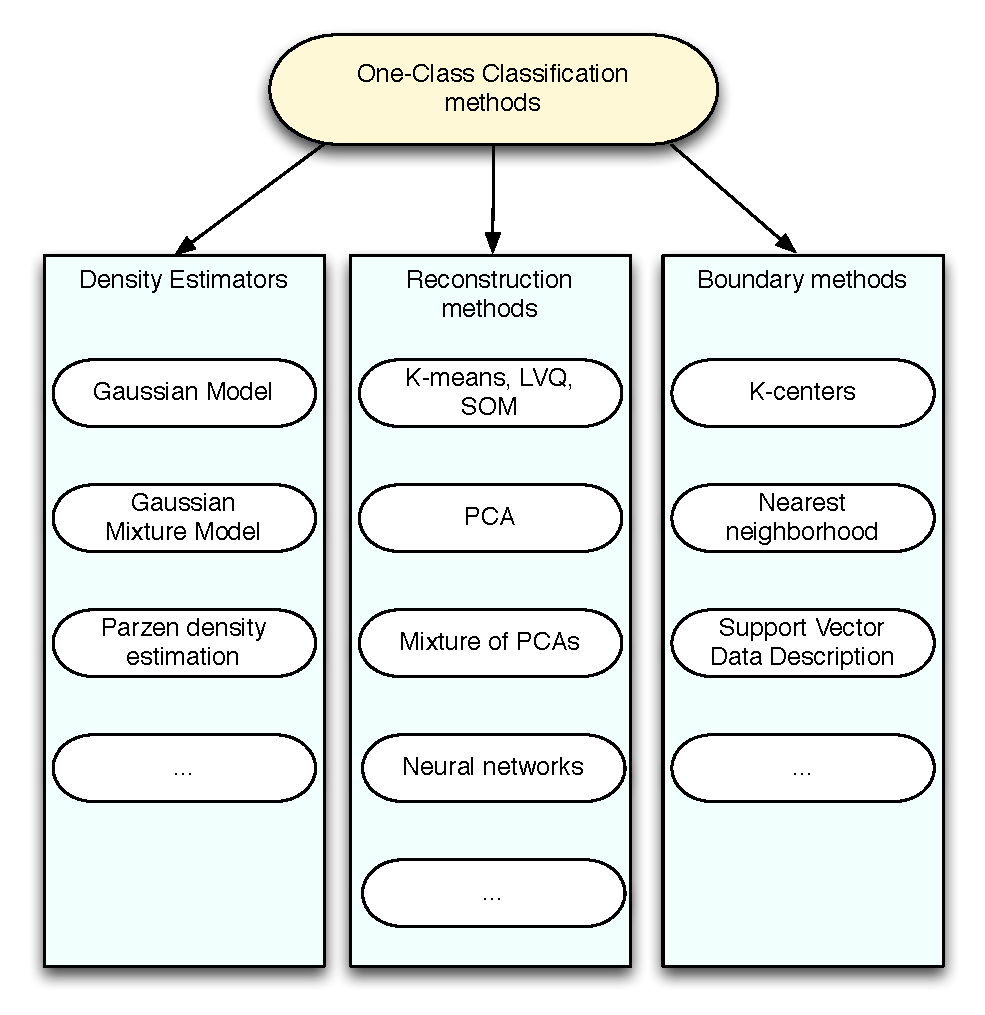
\includegraphics[width=0.5\textwidth,keepaspectratio]{./Figures/chapter3/occ_methods.pdf}
  \caption[\gls{occ} methods]{Overview of \gls{occ} methods categorized in Density Estimators, Reconstruction methods and Boundary methods. This categorization follows the definition of Tax in \cite{tax2001one}.}
  \label{fig:occ-methods}
\end{figure}

\subsection{Problem formulation}\label{subsec:occ-problem-formulation}
*** Introduce problem of \gls{occ}. Relate to two-class classification. ***

\subsection{One-Class Classification methods}\label{subsec:occ-methods}
In his thesis \cite{tax2001one}, Tax orders a collection of \gls{occ}-methods into three categories, visually represented in Figure \ref{fig:occ-methods}.
The first category consists of methods that estimate the density of the training data and set a threshold on this density.
Among those are Gaussian models, \glspl{gmm} and Parzen density estimators.
In order to get good generalization results with these methods, the dimensionality of the data and the complexity of the density need to be restricted.
This can cause a large bias on the data.
When a good probablity model is assumed, these methods work very well, since when one threshold is optimized, a minimum volume is automatically found for the given probability density model \cite{tax2001one}.

\subsection{Support Vector Data Description}\label{subsec:occ-svdd}
*** Short introduction of \gls{svdd}. More details in \ref{subsec:oc-svm-svdd}. ***

*** TODO: end with bridge to next chapter, \gls{oc-svm} ***

-- Literature --

``A survey of recent trends in one class classification'' \cite{khan2010survey}. 25, 2010 \\

``One-class classification by combining density and class probability estimation'' \cite{hempstalk2008one}. 51, 2008 \\

``On simple one-class classification methods'' \cite{noumir2012simple}. 2012 \\

``One-class classification'' \cite{tax2001one}. 693, 2001 \\

``The One-Class Classification Approach to Data Description and to Models Applicability Domain'' \cite{baskin2010one}. 19, 2009 \\

``One-class classifier networks for target recognition applications'' \cite{moya1993one}. 70, 1993. Origin of term ``One-Class Classification'' \\